\section{Positionsbestimmung}
\label{sec:GPS}
Um die geografische Lage des Autos festzuhalten, wird ein \ac{GPS}-Modul verwendet. Das System \ac{GPS} wird in Sektion \ref{subsec:tGPS} erklärt. Dazu gehört die Wahl der Elektronik, die Montage sowie die programmatische Implementation.

\subsection{Wahl der GPS-Elektronik}
\label{subsec:GPSchoice}
Das GY-NEO6MV2 \ac{GPS}-Modul mit Keramikantenne bietet eine günstige Möglichkeit zur Positionsbestimmung. Mit einer Genauigkeit von 1,5 bis 6 Metern, liefert es die Positionsdaten über die \ac{UART}-Schnittstelle, mithilfe des \ac{NMEA}-Protokolls. Näheres zur Datenübertragung wird in Sektion \ref{subsec:GPSprogram} erklärt. Die Wiederholungsrate der Datenpakete liegt standardmäßig bei 1 \ac{Hz} und kann auf bis zu 5 \ac{Hz} erhöht werden. Die Standard-Baudrate über die serielle Schnittstelle beträgt 9600 $\frac{\mathrm{\ac{b}}}{\mathrm{\ac{s}}}$. Versorgt wird das GY-NEO6MV2 mit 2.7 bis 5 V und arbeitet in einem Temperaturbereich von -40°C bis 85°C. Es hat eine Kaltstart-Zeit von 27 Sekunden und eine Hotstart-Zeit von 1 Sekunde. Ein Kaltstart ist bei einem GPS-Gerät die erste Erfassung von Satellitenbahnen und Zeiten bei der ersten Aktivierung, oder wenn sich das Gerät von der letzten Ortsbestimmung weit entfernt hat. Ein Hotstart tritt bei einer Aktivierung des GPS-Moduls dann auf, wenn es die Satellitendaten noch weiß. Das ist meistens der Fall, wenn nicht mehr als sechs Stunden seit der letzten Positionserfassung vergangen sind und sich das Gerät seit dem nicht weit entfernt hat. Die angegebenen Zeiten sind dabei die kleinstmöglichen. Die dazugehörige Keramikantenne wird über eine UFL-Hirose-Verbindung am GPS-Modul angesteckt. 

\subsection{Montage der GPS-Elektronik}
\label{subsec:GPSmount}
Das GY-NEO6MV2 Modul ist an der Innenseite des Deckels des Elektronikgehäuses mit doppelseitigem Klebeband angebracht. Der Vorteil dieser Montagestelle ist die Fixiermöglichkeit der Antenne. Diese muss, um Satelliten-Daten empfangen zu können, in den freien Himmel zeigen. Über eine Bohrung im Deckel des Gehäuses der Elektronik ist die Antenne mit der Platine verbunden.

\subsection{Programmatische Implementation}
\label{subsec:GPSprogram}
Wie bereits erwähnt liefert das GPS-Modul die Daten über die UART-Schnittstelle. Dabei wird die transmit (TX)-Leitung des GPS-Moduls mit dem receive (RX)-Pin des Raspberry Pi verbunden. Die receive-Leitung des Moduls ist nicht nötig, da es nur die Daten an den \ac{Raspi} senden soll.\\
Um den seriellen (\ac{UART}) Port des Raspberry Pi verwenden zu können muss dieser zunächst in der Konfigurationsdatei  \verb|/boot/config.txt| mit dem Hinzufügen der Zeile \verb|enable_uart=1| aktiviert werden. Des Weiteren muss die Konsole \glqq getty\grqq\ der seriellen Schnittstelle \verb|/dev/ttyAMA0| deaktiviert werden, um diese in einem Python Programm einbinden zu können. Dazu ist einerseits der Befehl \verb|sudo systemctl stop serial-getty@ttyAMA0.service|\ notwendig, um den Prozess zu stoppen, andererseits muss der Befehlt \verb|sudo systemctl disable serial-getty@ttyAMA0.service| verwendet werden, um das automatische Initialisieren des Prozesses durch systemd zu unterbinden.\\
Das \ac{GPS}-Modul gibt die Daten mit dem \ac{NMEA}-Protokoll, welches der Standard in der GPS-Technik ist, an den Raspberry Pi weiter. Der Inhalt eines Datenpaketes in diesem Format sieht wie in Abbildung \ref{fig:NMEA} dargestellt aus. Wie zu erkennen ist, bestehen diese \ac{GPS}-Daten aus mehreren \ac{GPS}-Nachrichten. Jede dieser verschiedenen Nachrichten (Zeilen) wird durch einen sogenannten Protokoll-Header gekennzeichnet. Diese sind GPGGA, GPGSA, GPGSV, GPGLL, GPRMC und GPVTG. Nachfolgend an den Header stehen die verschiedenen Informationen mit Komma getrennt. Dieses Format hat sich gerade deswegen durchgesetzt, da es eine Vielzahl an Informationen beinhaltet und es dem Programmierer überlassen ist, welche Informationen er davon verwenden möchte. Bei den unterschiedlichen Headern sind die Daten verschieden, beziehungsweise in einer anderen Reihenfolge angeordnet. Der Header GPRMC wird hier verwendet, da er die Längen- und Breitengrade klar erkenntlich und einfach beinhaltet. Die Inhalte und Reihenfolge der Daten ist folgendermaßen aufgebaut: An erster Stelle befindet sich die koordinierte Weltzeit (UTC) in jeweils zweistelligen Stunden, Minuten und Sekunden. Danach folgt der Status. Ein A steht für \glqq data valid\grqq , ein V für \glqq data not valid\grqq . An der nächsten Stelle steht der Breitengrad (latitude), danach folgt die Kennzeichnung mit einem N oder S für \glqq nördliche oder südliche Breite\grqq . Der Längengrad (longitude) steht als nächstes, mit der Kennzeichnung W oder E für \glqq westliche oder östliche Länge\grqq . Die Einheit der Längen- und Breitengrade ist dabei Grad und anschließend Minuten als Dezimalzahl. Die Positionsdaten 4728.545 N, 01524.038 E entsprechen beispielsweise den Koordinaten 47° 28.545' N und 15° 24.038' E.

\begin{figure}[h]
\centering
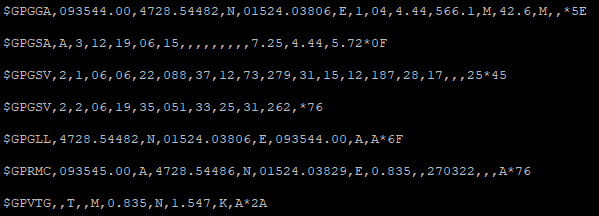
\includegraphics[scale=0.8]{NMEA.png}
\caption{Daten des GPS-Moduls im NMEA-Format}
\label{fig:NMEA}
\end{figure}

Um diese Positionsdaten programmatisch herauszufiltern, wird jede GPS-Nachricht auf ihre ersten sechs Zeichen überprüft. sollten diese \verb|$GPRMC| entsprechen, wird mithilfe der pynmea2 Bibliothek, wie in Sektion \ref{subsubsec:tpynmea2} beschrieben, die Daten der Breiten- und Längengrade auf zwei Variablen geschrieben. Diese Positionsdaten werden automatisch in Grad als Dezimalzahl formatiert. 